\hypertarget{population_8h}{
\section{Referencia del Archivo population.h}
\label{population_8h}\index{population.h@{population.h}}
}


\subsection{Descripci\'{o}n detallada}
Declaraciones del Objeto Poblacion 

Definici\'{o}n en el archivo \hyperlink{population_8h-source}{population.h}.

{\tt \#include \char`\"{}individuo.h\char`\"{}}\par
{\tt \#include \char`\"{}genesting.h\char`\"{}}\par


Dependencia gr\'{a}fica adjunta para population.h:\begin{figure}[H]
\begin{center}
\leavevmode
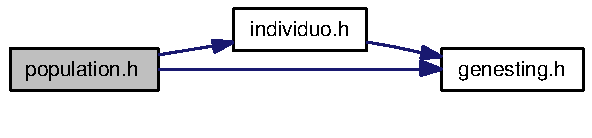
\includegraphics[width=160pt]{population_8h__incl}
\end{center}
\end{figure}


Este gr\'{a}fico muestra que archivos directa o indirectamente incluyen a este archivo:\begin{figure}[H]
\begin{center}
\leavevmode
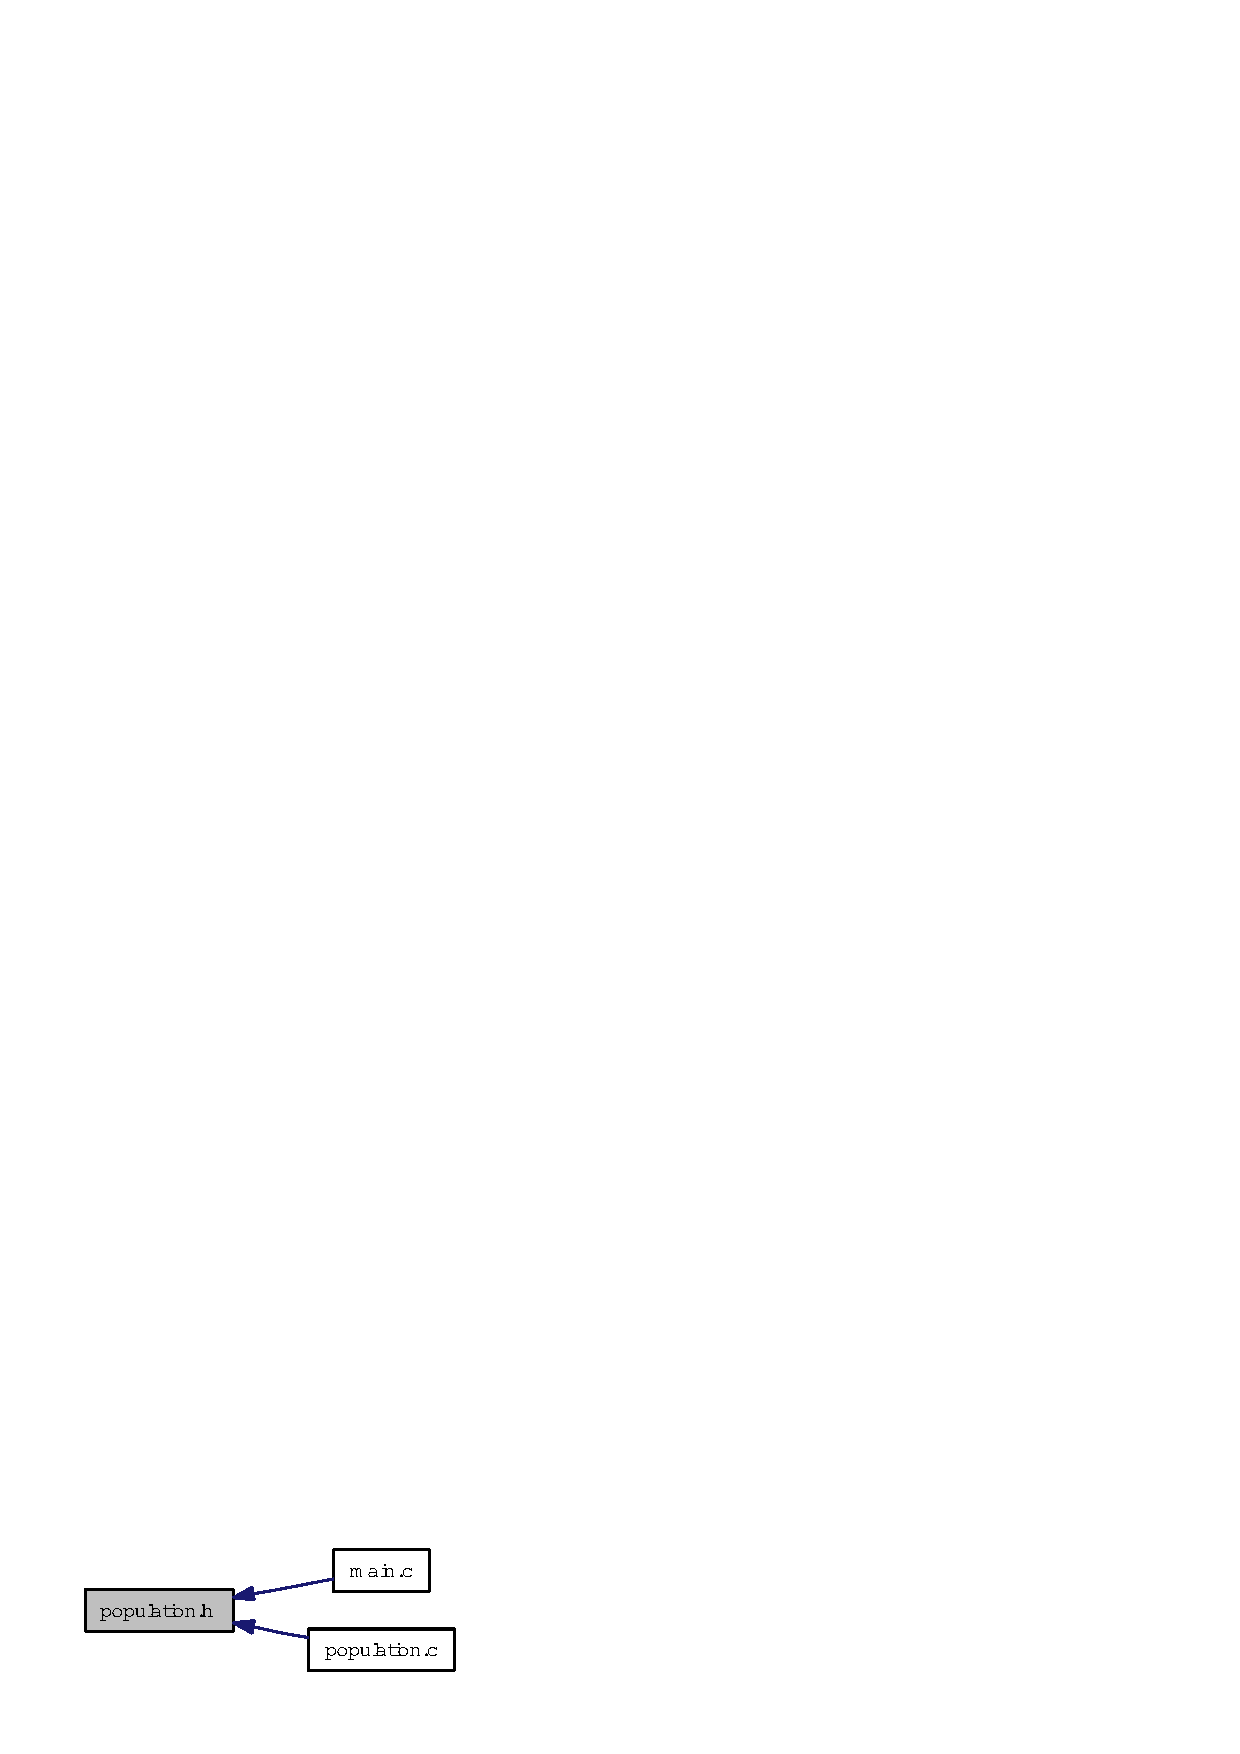
\includegraphics[width=111pt]{population_8h__dep__incl}
\end{center}
\end{figure}
\subsection*{Clases}
\begin{CompactItemize}
\item 
struct \hyperlink{struct__population}{\_\-population}
\end{CompactItemize}
\subsection*{Tipos definidos}
\begin{CompactItemize}
\item 
typedef \hyperlink{struct__population}{\_\-population} \hyperlink{group__genetic_gdc93697b2d7197da72db59932b540a07_gdc93697b2d7197da72db59932b540a07}{population}
\end{CompactItemize}
\subsection*{Funciones}
\begin{CompactItemize}
\item 
void \hyperlink{group__genetic_gc7ba874876f18abab66f0a42f32b98cc_gc7ba874876f18abab66f0a42f32b98cc}{population\_\-create} (\hyperlink{struct__population}{population} $\ast$p, \hyperlink{struct__genesting}{genesting} $\ast$g, int n)
\item 
void \hyperlink{group__genetic_g229293c432c5ef4f70b1ee94c109bb1a_g229293c432c5ef4f70b1ee94c109bb1a}{population\_\-evaluate} (\hyperlink{struct__population}{population} $\ast$p)
\item 
void \hyperlink{group__genetic_g5b3202f02e14d7fb3eb1f729d1250243_g5b3202f02e14d7fb3eb1f729d1250243}{population\_\-generation} (\hyperlink{struct__population}{population} $\ast$p)
\end{CompactItemize}
